
\begin{figure}[ptb]

\includegraphics[scale=0.30]{logo.jpg}\hspace{6cm}

\includegraphics[scale=0.90]{logo_dc.jpg}
\end{figure}

%Datos de la caratula
\materia{M\'etodos Num\'ericos}
\titulo{Trabajo pr\'actico 2}
\subtitulo{Tu cara me suena}
\hspace{6cm}
\begin{minipage}[b]{0.5\linewidth}
\begin{figure}[H]
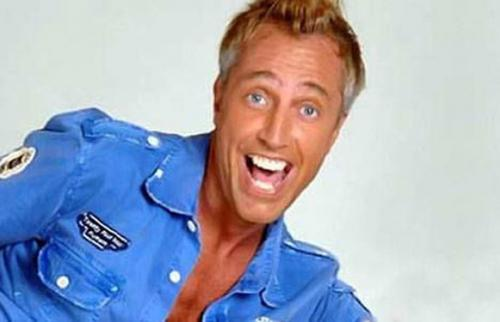
\includegraphics[scale=0.10]{marley.jpg}\hspace{6cm}
\end{figure}
\end{minipage}
\integrante{Gandini, Luciano}{207/10}{gl.gandini@gmail.com}
\integrante{Russo, Christian Sebastián}{679/10}{christian.russo@gmail.com}
\integrante{Danós, Alejandro}{381/10}{adp007@gmail.com}
\resumen{El presente trabajo documenta un algoritmo de reconocimiento de rostros para sujetos
  pertenecientes a una base de datos. Hace uso de un Análisis de Componentes Principales (PCA según
  sus siglas en inglés) sobre un conjunto de imágenes digitales de rostros de sujetos. Se alega
  poder identificar con una tasa de error mínima una nueva imagen de un rostro de una persona
  perteneciente a la base de datos. Se explican los supuestos matemáticos asumidos en el algoritmo,
se muestran resultados de diferentes pruebas de su efectividad y se llega a conclusiones sobre todo
el proceso.}
\palabrasClave{Reconocimiento caras. PCA. Power Method. Deflation. Autovalores. Autovectores. Matriz
  semi definida positiva.}
% \resumen{El presente trabajo analiza los algor\'itmos de resoluci\'on de sistemas de ecuaciones %
% Gauss y LU mediante una simulaci\'on del c\'alculo de Isotermas en hornos industriales. \\ %
% Expone un sistema de ecuaciones para detectar la Isoterma de 500 grados y analiza el
% comportamiento de cada algoritmo en funci\'on a la discretizaci\'on de los puntos dentro del
% horno, cantidad de instancias a resolver y variaci\'on de instantes.\\ % Finalmente, detalla las
% conclusiones obtenidas mediante la comparaci\'on de ambos algoritmos en las circunstancias
% mencionadas.\\ 
% }
\hypersetup{%
 % Para que el PDF se abra a página completa.
 pdfstartview= {FitH \hypercalcbp{\paperheight-\topmargin-1in-\headheight}},
 pdfauthor={Gandini, Russo, Danós},
 pdfsubject={TP1}
}

\parskip=5pt % 10pt es el tamaño de fuente

% Pongo en 0 la distancia extra entre ítemes.
\let\olditemize\itemize
\def\itemize{\olditemize\itemsep=0pt}

% Acomodo fancyhdr <- Creo que es el encabezado de pagina
\pagestyle{fancy}
\thispagestyle{fancy}
\addtolength{\headheight}{1pt}
\lhead{M\'etodos Num\'ericos, TP2 - Gandini, Russo, Danós}
\rhead{1$^{er}$ Cuatrimestre 2014}
\cfoot{\thepage}
\renewcommand{\footrulewidth}{0.4pt}




%Pagina de titulo e indice
\thispagestyle{empty}

\maketitle
\tableofcontents

\newpage

